\documentclass[a4paper,onecolumn,10pt]{article}
\usepackage[polish]{babel}
\usepackage[utf8]{inputenc}
\usepackage[T1]{fontenc}
\usepackage[left=2.1cm,right=2.1cm]{geometry}
\usepackage[dvipsnames]{xcolor}
\usepackage{amsmath,calc,indentfirst,fancyhdr,amsfonts,graphicx,epstopdf,caption, mathcomp, subcaption,wrapfig, siunitx,pbox,float,algorithm}
\usepackage[noend]{algpseudocode}


\makeatletter
\def\BState{\State\hskip-\ALG@thistlm}
\renewcommand{\ALG@name}{Algorytm}
\makeatother

\renewcommand{\baselinestretch}{1.1}	 % odstep miedzy liniami
\addto\captionspolish{\renewcommand{\figurename}{Wykres}} % zmiana podpisu pod obrazkami, zamiast "Rysunek" bedzie "Wykres"
\newcommand{\NN}{\mathbb{N}}			 % makro do znaku liczb naturalnych

\newcommand{\R}[1]{\textcolor{red}{#1}}  % makro do polecenia z parametrami - tutaj 1 parametr
\newcommand{\G}[1]{\textcolor{green}{#1}} 
\newcommand{\B}[1]{\textcolor{RoyalBlue}{#1}} 
% kolorowanie {\B{argument}}

\newcommand{\PICTURES}{} % szybsza kompilacja dzieki stalej "usuwajacej" obrazki
						 % zakomentowanie \PICTURES powoduje znikniecie obrazkow

\pagestyle{fancy} % formatuj caly dokument
\fancyhead{}
\fancyfoot{}
\renewcommand{\headrulewidth}{0pt}
\fancyfoot[R]{\thepage} % dla stron poza tytulowa nr w prawym dolnym rogu

\fancypagestyle{plain}{ % dla strony tytulowej nr w prawym dolnym rogu
	
	\renewcommand{\headrulewidth}{0pt}
	\fancyhf{}
	\fancyfoot[R]{\thepage}
}

\title{\Large\vspace{-2.5cm}{\Huge S}PRAWOZDANIE - LABORATORIUM NR {\Huge1}\\
		\textbf{Rozwiązywanie układu równań liniowych \\metodami bezpośrednimi} } 
\date{\Large28 lutego 2019}
\author{\Large Marek Kiełtyka}

\begin{document}
\maketitle

\section{Wstęp}
	
\subsection{Metoda Gaussa-Jordana}

Metoda ta znajduje zastosowania w algebrze. Za jej pomocą można obliczać macierze odwrotne oraz znacząco uprościć rozwiązywanie układów równań liniowych, co wykorzystano podczas niniejszego laboratorium. Aby to osiągnąć, należy zapisać dany układ w\,postaci macierzowej:
\begin{equation}
\begin{pmatrix}
a_{1,1} & a_{1,2}  & \dots  & a_{1,n} \\
a_{2,1} & a_{2,2}  & \dots  & a_{2,n} \\
\vdots & \vdots & \ddots & \vdots \\
a_{n,1} & a_{n,2}  & \dots  & a_{n,n}
\end{pmatrix}
\cdot
\begin{pmatrix}
x_{1} \\
x_{2} \\
\vdots \\
x_{n}
\end{pmatrix}
= 
\begin{pmatrix}
b_{1} \\
b_{2} \\
\vdots \\
b_{n}
\end{pmatrix}
\label{macierzrownan}
\end{equation}
gdzie macierz $ \boldsymbol{A} $ (tzw. podstawowa) i wektory $ \boldsymbol{x}, \boldsymbol{b} $ oznaczają kolejno: \begin{itemize}
	\item współczynniki - $a_{i,j}$,
	\item niewiadome - $x_i$
	\item wyrazy wolne - $b_i$
\end{itemize}
Dalej należy stosować opisane poniżej operacje. 

\subsubsection{Rozwiązywanie URL}
W celu uzyskania rozwiązania należy zestawić macierze w sposób: $ \left[ \boldsymbol{A}\right]\left[\boldsymbol{b}\right] $. Następnie korzystając z dozwolonych operacji, tj.
\begin{itemize}
	\item mnożenia wierszy przez liczbę różną od zera,
	\item dodawania i odejmowania wierszy do siebie,
\end{itemize}
manipulujemy zawartością macierzy do momentu osiągnięcia $a_{i,j} = 
 \begin{cases}
	1,& i = j \\
	0,& i \neq j 
\end{cases} $, tj. macierzy jednostkowej $ \boldsymbol{I}. $ Wtedy wektor $ \boldsymbol{b_{rozw}} $ zawiera kolejne wartości poszukiwanych niewiadomych, zatem:
\begin{equation}
\boldsymbol{I} \cdot \boldsymbol{x} =  \boldsymbol{b_{rozw}}.
\end{equation}

\subsubsection{Wyznaczenie macierzy odwrotnej}
Tym razem dokonujemy takiego zestawienia $ \left[\boldsymbol{A}\right]\left[\boldsymbol{I}\right] $ - jeśli tylko wejściowa macierz jest odwracalna. Operując dozwolonymi sposobami na obu macierzach staramy się uzyskać macierz jednostkową w miejscu wejściowej. Na skutek tego po prawej stronie ukaże się poszukiwana macierz odwrotna. Końcowym rezultatem będzie $ \left[\boldsymbol{I}\right]\left[\boldsymbol{A^{-1}}\right]. $

\section{Zadanie do wykonania}

\subsection{Opis problemu}
Równania różniczkowe stanowią typowy przykład URL. Na laboratorium poruszono tematykę oscylatora harmonicznego, dla którego z II zasady dynamiki Newtona wynika:
\begin{equation}
\frac{\partial^2 x(t)}{\partial t^2} = - \frac{k}{m} x(t) = -\omega^2 x(t)
\label{oscylator}
\end{equation}
Można dokonać prostego przybliżenia przy pomocy ilorazu różnicowego, uzależniając drugą pochodną położenia \textit{x} w chwili \textit{t} wyłącznie od tych parametrów.
\begin{equation}
\frac{\partial^2 x(t)}{\partial t^2} \approx \frac{x(t+\Delta t) - 2x(t) + x(t - \Delta t)}{(\Delta t)^2}
\end{equation}
Oznaczając odpowiednio $\Delta t = h$ oraz $x_i = x(ih)$ otrzymamy z równania (\ref{oscylator}) iteracyjną metodę obliczania kolejnych położeń $x_i$.
\begin{equation}
x_{i+1} +(\omega^2 h^2 - 2)x_i + x_{i+1} = 0
\label{iteracyjnie}
\end{equation}
Założenia początkowe:
\begin{alignat*}{6}
	x_0 = A = 1 &- \text{ początkowe wychylenie z położenia równowagi} \\
	\omega = \sqrt{\frac{k}{m}} = 1 &- \text{ częstość kołowa} \\
	v_0 = \frac{x_1 - x_0}{h} = 0 &- \text{ prędkość początkowa} \\
	h = 0,1 &- \text{ krok całkowania} \\
	N = 400 &- \text{ ilość kroków całkowania.}
\end{alignat*}

Zasadniczym problemem było wyznaczenie położenia w kolejnych krokach czasowych i sporządzenie wykresu tej zależności na podstawie wyniku. Zapisując równanie (\ref{iteracyjnie}) w\,ogólnej postaci macierzowej można było skorzystać z metody Gaussa-Jordana w\,celu rozwiązania układu (\ref{ogolna}).

\begin{equation}
\begin{pmatrix}
1      & 0 				 & 0      &\dots  			& 0  \\
-1     & 1               & 0      &\dots  			& 0  \\
1  	   & (\omega^2h^2-2) & 1      &\dots  			& 0  \\
\vdots & \ddots          & \ddots &\ddots 			& 0  \\
0      & 0               & 1 	  &(\omega^2h^2-2)  & 1  \\
\end{pmatrix}
\cdot
\begin{pmatrix}
x_0 \\
x_1 \\
x_2 \\
\vdots \\
x_n
\end{pmatrix}
= 
\begin{pmatrix}
A \\
v_0h \\
0 \\
\vdots \\
0
\end{pmatrix}
\label{ogolna}
\end{equation}

\subsection{Wyniki}
Korzystając z biblioteki \textit{numutil} i gotowej procedury: \begin{center}
	\textit{void gaussj(float **a, int n, float **b, int m);}
\end{center}
napisano program w języku C++ w celu rozwiązania opisanego problemu. Otrzymane na wyjściu kroki czasowe i odpowiadające im wartości wychylenia z położenia równowagi należało umieścić na wykresie, co znacząco ułatwiło interpretację wyniku. Było to rozwiązanie numeryczne, które porównano z rozwiązaniem analitycznym (dla oscylatora harmonicznego jest to przebieg funkcji $ cosinus $).

\begin{figure}[h]
	\begin{center}
		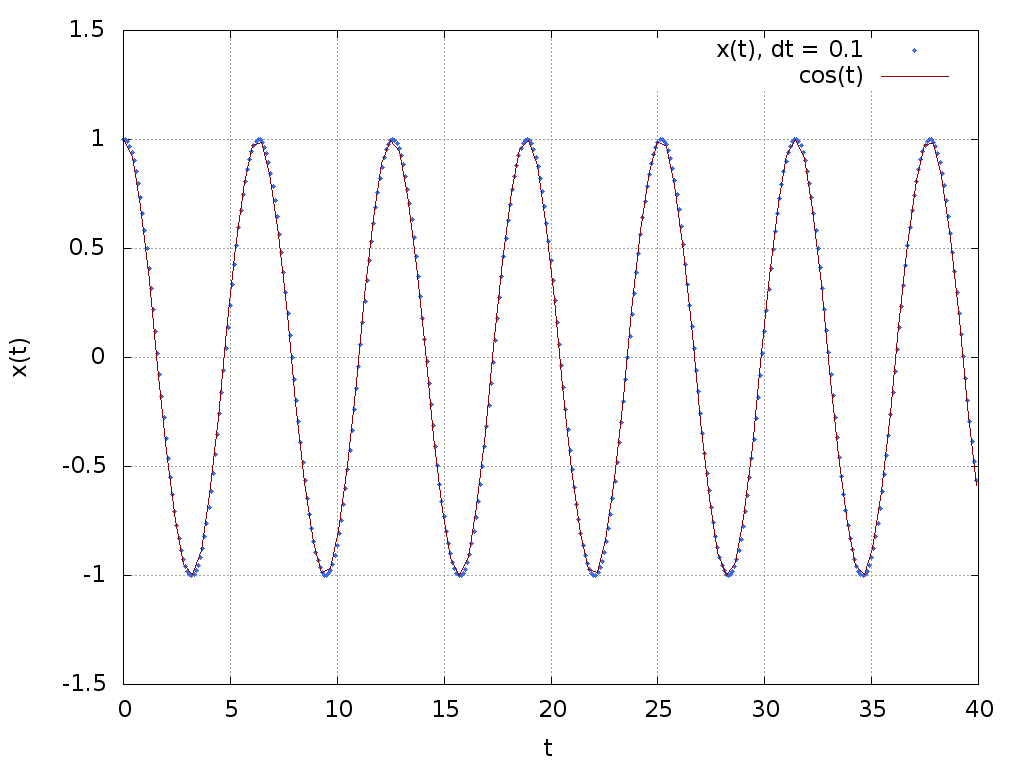
\includegraphics[width=1.0\textwidth]{wychylenie.png}
		\caption{Wychylenie $x(t)$.}
		\label{wykres}
	\end{center}
\end{figure}

\newpage
\section{Wnioski}
Wykres (\ref{wykres}) prezentuje niemal idealne pokrycie rozwiązań uzyskanych odmiennymi metodami. Trend utrzymuje się na przestrzeni kilku okresów drgań, więc stwierdzamy, iż w przypadku zwiększenia ilości kroków czasowych rozwiązanie wciąż będzie poprawne. Nieznaczne rozbieżności można by niwelować dalej poprzez stopniowe skracanie pojedynczego kroku. W rezultacie otrzymalibyśmy równocześnie większe zagęszczenie punktów oraz lepsze dopasowanie. Podsumowując, metoda Gaussa-Jordana jest bardzo dobrym narzędziem do rozwiązywania układów równań liniowych, gwarantującym wysoką dokładność rezultatów.


\end{document}